%------------------------------------------------------------------%
% Cannabis Data Science Presentation 3/17/2021
%
% FIXME: Bibliography
% https://tex.stackexchange.com/questions/148893/package-biblatex-error-incompatible-package-ucs-begindocument?noredirect=1&lq=1
% https://tex.stackexchange.com/questions/261595/how-to-rerun-biber-on-the-file
% https://tex.stackexchange.com/questions/229638/package-biblatex-warning-babel-polyglossia-detected-but-csquotes-missing
% https://tex.stackexchange.com/questions/49610/use-biblatex-and-utf8
% https://stackoverflow.com/questions/1507672/putting-citation-text-on-same-slide-with-latex-beamer
%------------------------------------------------------------------%
\documentclass[xcolor={dvipsnames}]{beamer}
\hypersetup{pdfpagemode=FullScreen}
\mode<presentation> %TEMPLATE
{ \usetheme{Boadilla}
  \usecolortheme{orchid}
  \usefonttheme{default}
  \setbeamertemplate{navigation symbols}{}
  \setbeamertemplate{caption}[numbered]} 
\usepackage[english]{babel}
\usepackage[utf8x]{inputenc}
\setbeamersize{text margin left=0.5in,text margin right=0.5in}

\usepackage[dvipsnames]{xcolor}
\definecolor{DarkGreen}{RGB}{2, 48, 32}
\definecolor{CalyxGreen}{RGB}{34, 153, 84}
\definecolor{DarkOrange}{RGB}{199, 0, 57}
\definecolor{LightOrange}{RGB}{255, 87, 51}
\definecolor{LightGreen}{RGB}{218, 247, 166}
\definecolor{LightYellow}{RGB}{255, 195, 0}

\setbeamercolor*{palette primary}{bg=LightGreen, fg = DarkGreen}
\setbeamercolor*{palette secondary}{bg=LightGreen, fg=DarkGreen}
\setbeamercolor*{palette tertiary}{bg=LightGreen, fg = DarkGreen}
%\setbeamercolor*{palette quaternary}{bg=myNewColorD, fg = green}

%------------------------------------------------------------------%
% FIXME: Bibliography
%------------------------------------------------------------------%
%\usepackage{csquotes}
%\usepackage[style=verbose]{biblatex}
%\addbibressource{presentation-bib.bib}

%------------------------------------------------------------------%
% Packages
%------------------------------------------------------------------%
\usepackage{amsmath}
\renewcommand*\footnoterule{} %No sperating line on footnote
\usepackage{mathtools} %ANNOTATING EQUATIONS
\usepackage{hhline} %DOUBLBARS
\newcommand\T{\rule{0pt}{2.5ex}} %TOPSTRUT
\newcommand\B{\rule[-1.25ex]{0pt}{0pt}} %BOTTOMSTRUT
\newenvironment<>{varblock}[2][.9\textwidth] %RESIZED BLOCKS
  {\setlength{\textwidth}{#1}
  \begin{actionenv}#3
    \def\insertblocktitle{#2}\par
    \usebeamertemplate{block begin}}
  {\par\usebeamertemplate{block end}
  \end{actionenv}}
\defbeamertemplate{enumerate item}{largeball} %LARGE BALLS
{\begin{pgfpicture}{-1ex}{-0.65ex}{1.5ex}{1.5ex}
\usebeamercolor[fg]{item projected}
{\pgftransformscale{2.5}\pgftext{\Large\pgfuseshading{bigsphere}}}
{\pgftransformshift{\pgfpoint{0pt}{0.5pt}}
\pgftext{\usebeamerfont*{item projected}\small\insertenumlabel}}
\end{pgfpicture}}
\usepackage{tikz} % FANCY ARROWS
\usepackage{xparse}
\NewDocumentCommand\UpArrow{O{2.0ex} O{black}}{%
   \mathrel{\tikz[baseline] \draw [->, line width=0.5pt, #2] (0,0) -- ++(0,#1);}} % FANCY UPARROW
\NewDocumentCommand\DownArrow{O{2.0ex} O{black}}{%
   \mathrel{\tikz[baseline] \draw [<-, line width=0.5pt, #2] (0,0) -- ++(0,#1);}} % FANCY DOWNARROW
%\vskip 1cm
\makeatletter
\newcommand{\LeftEqNo}{\let\veqno\@@leqno}%LEFT EQUATION #'s
\makeatother

%------------------------------------------------------------------%
% Title
%------------------------------------------------------------------%
\title[Meetup]{}
\author{Cannabis Data Science}
\institute[]{\Large Meetup}
\date{March 17, 2021}
\begin{document}
\begin{frame}{}
  
\includegraphics[scale=0.075]{images/logos/cannlytics_logo_with_text_light.png}
  \titlepage
\end{frame}

%------------------------------------------------------------------%
% Introduction
%------------------------------------------------------------------%
\section{Introduction}

\begin{frame}{}

The `licit--yet--illegal' status of the cannabis industry allows for land and finance owners to extract high risk--based rents from land and capital loans.
\vspace{1\baselineskip}

{\scriptsize Polson, M. (2013), ‘Land and Law in Marijuana Country: Clean Capital, Dirty Money, and the Drug War’s Rentier Nexus’, PoLAR: Political and Legal Anthropology Review 36(2), 215.}

\end{frame}

% Production function
\begin{frame}{}
Suppose that the total amount of cannabis sold in a given period, $y_t$, is a simple function of the number of plants cultivated that period, $k_t$,

$$y_t = Ak_t^\alpha\mathrm{e}^{\varepsilon_t},$$

where $A$ represents the state of cultivation technology and $\varepsilon_t$ is a random production shock.
\end{frame}

% Production charts
\begin{frame}{}
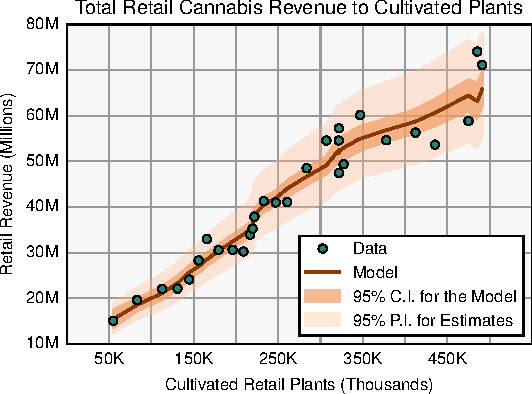
\includegraphics[scale=0.5]{images/revenue-to-plants-retail.pdf}
\hspace{2ex}
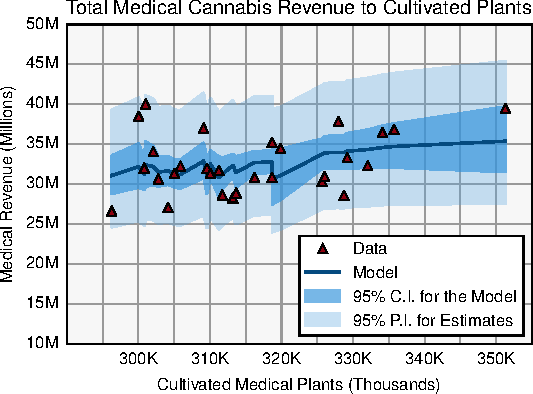
\includegraphics[scale=0.5]{images/revenue-to-plants-medical.pdf}
\vspace{1\baselineskip}

Economic theory suggests that the production function should have diminishing marginal returns, such that $ 0 \leq \alpha < 1$.
\end{frame}

% Estimation
\begin{frame}{}
The production function can be estimated after a linear transformation

$$\ln y_t = \ln A + \alpha \ln k_t + \varepsilon_t.$$

You can use the approximated area of cannabis cultivation as a proxy for the amount of capital, $k_t$, in any given month.
\end{frame}


% Rate of return
\begin{frame}{}
The competitive rate of return on capital is equal to its marginal productivity minus depreciation
$$r_{K,t} = \alpha k_t^{\alpha -1} - \delta,$$
where $\delta$ is the monthly depreciation rate of capital required in cannabis production.
\end{frame}


% Empirical rate of return
\begin{frame}{}
The interest rates on money loans from financial lenders to cannabis business are typically higher than the market rates for comparable businesses, with interest rates usually between 7\% and 15\%.
\vspace{1\baselineskip}

{\scriptsize Polson, M. (2013), ‘Land and Law in Marijuana Country: Clean Capital, Dirty Money, and the Drug War’s Rentier Nexus’, PoLAR: Political and Legal Anthropology Review 36(2), 215.}
\end{frame}

%------------------------------------------------------------------%
% Takeaway
%------------------------------------------------------------------%

\begin{frame}{}
\begin{center}
\begin{minipage}{3.85in}
Thank you for coming.
\end{minipage}
\end{center}
\end{frame}

%----------------------------------------------------------------%
\end{document}
%------------------------------------------------------------------%